\chapter{Appendix 1: Analysis of the network embedding learned from local structural and time components}
\label{appendix:k-means_time}

\section{$k$-means}
~\autoref{fig:App1} shows learned and reduced by three dimensionality reduction techniques sets of embeddings. From~\autoref{fig:App2} and~\autoref{fig:App3} one may conclude the optimal $k$ for $k$-means: PCA - $k$ = 3; t-SNE - $k$ = 3; UMAP - $k$ = 3.~\autoref{fig:App4} demonstrates the clustering results on data sets from ~\autoref{fig:App1}. The best clustering according to the set of internal clustering metrics is UMAP-reduced embeddings split into 3 clusters (right plot on~\autoref{fig:App4}).

\begin{figure}[!ht]
	\centering
	\includegraphics[width=1.0\textwidth]{images/appendix/App1.pdf}\\
	\caption{Embeddings sets reduced to 3 dimensions by three dimensionality reduction techniques.}
	\label{fig:App1}
\end{figure}
\begin{figure}[!ht]
	\centering
	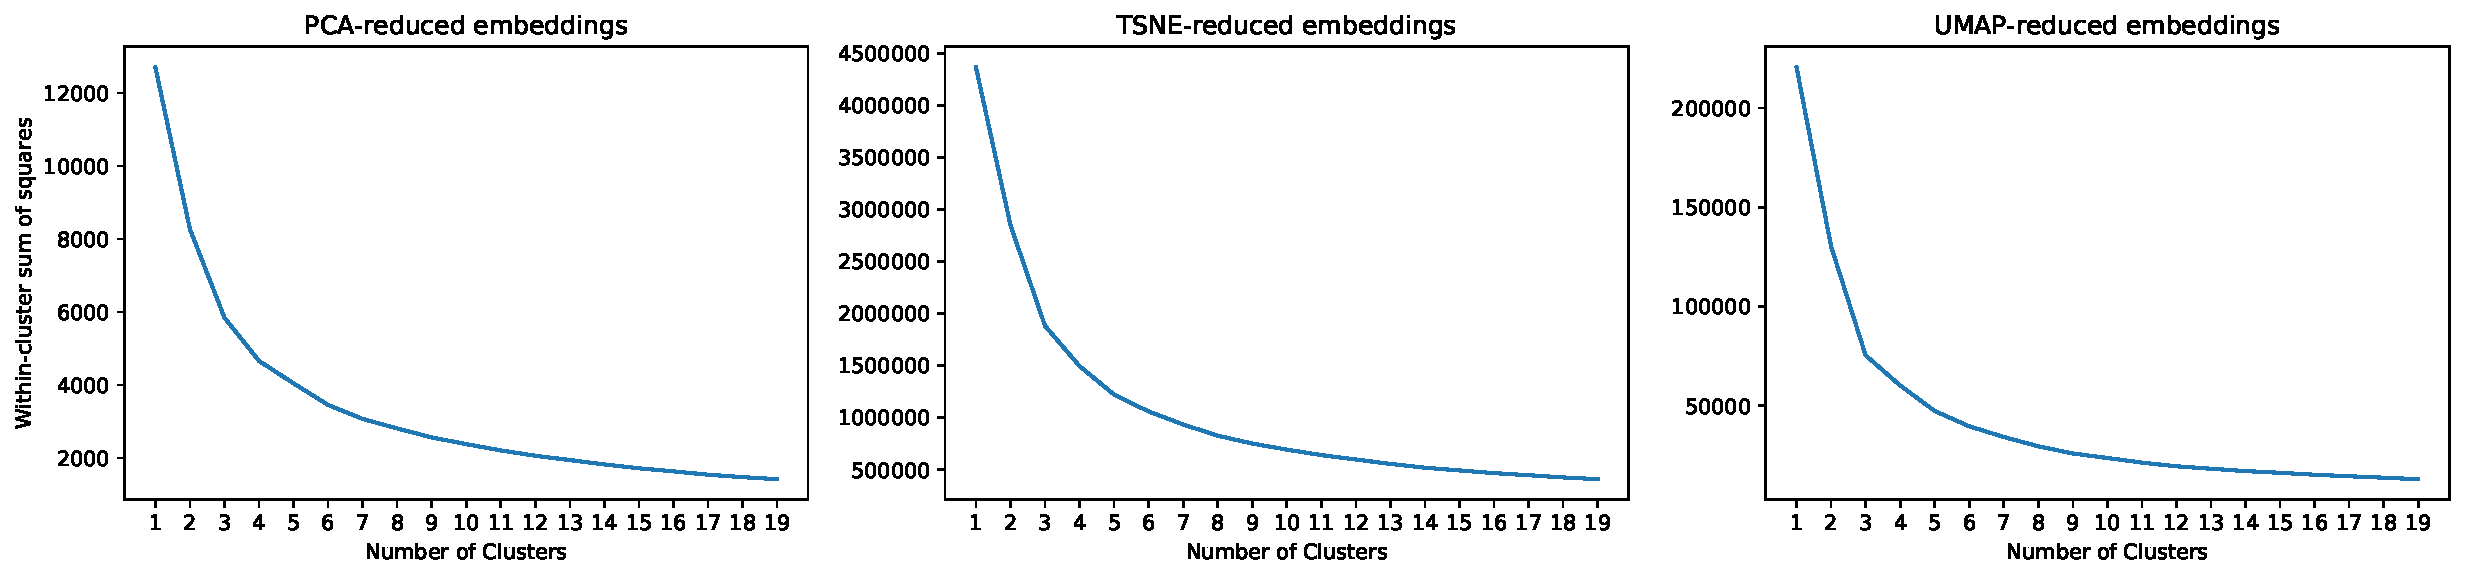
\includegraphics[width=1.0\textwidth]{images/appendix/App2.pdf}\\
	\caption{Elbow plots for 3-dimensional embedding sets.}
	\label{fig:App2}
\end{figure}
\begin{figure}[!ht]
	\centering
	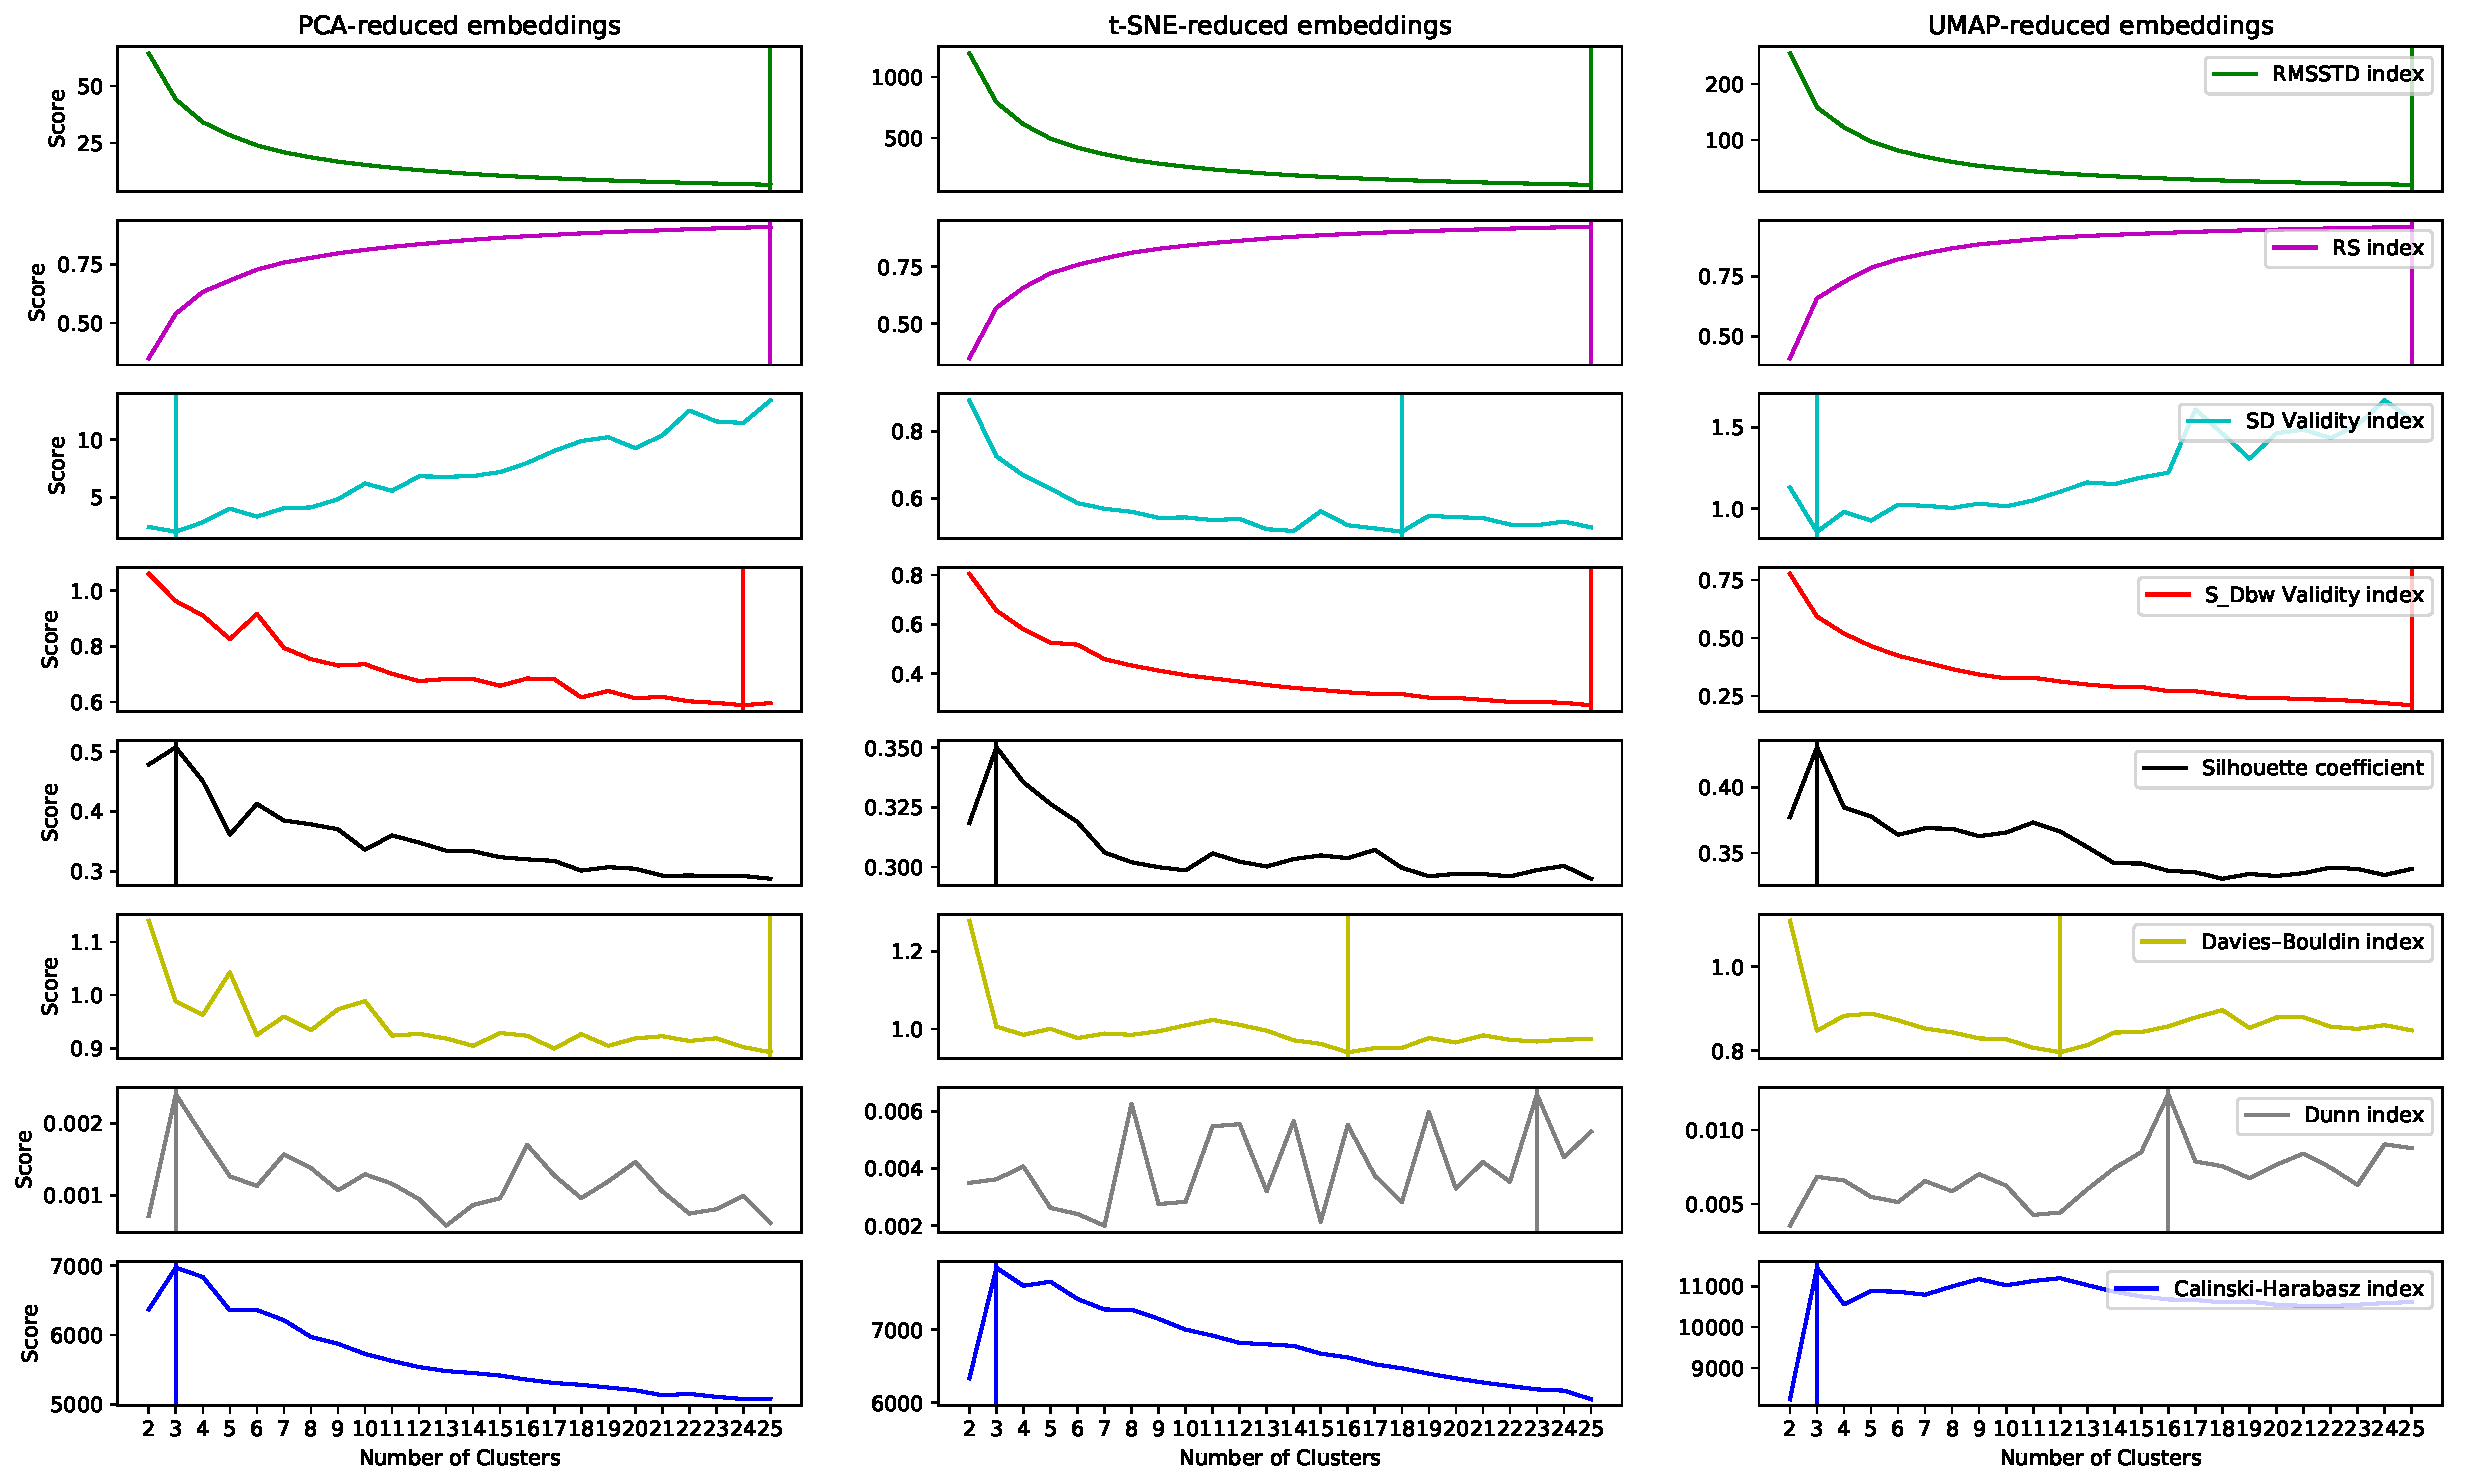
\includegraphics[width=1.0\textwidth]{images/appendix/App3.pdf}\\
	\caption{Evaluation of $k$-means clustering with respect to the number of clusters $k$.}
	\label{fig:App3}
\end{figure}
\begin{figure}[!ht]
	\centering
	\includegraphics[width=1.0\textwidth]{images/appendix/App4.pdf}\\
	\caption{Resulting $k$-means clustering.}
	\label{fig:App4}
\end{figure}

\section{HDBSCAN}

The sets from~\autoref{fig:App1} were clustered by HDBSCAN.~\autoref{fig:App9} suggests the best hyperparameters: PCA - min\_cluster\_size = 10, min\_samples = 5, alpha = 0.25;
t-SNE - min\_cluster\_size = 10, min\_samples = 5, alpha = 0.25; UMAP - min\_cluster\_size = 10, min\_samples = 40, alpha = 0.25.~\autoref{fig:App10} shows the coloured by defined HDBSCAN clusters embeddings. The best clustering according to the set of internal clustering metrics is t-SNE-reduced embeddings split into 2 clusters (middle plot on~\autoref{fig:App10}).

\begin{figure}[!ht]
	\centering
	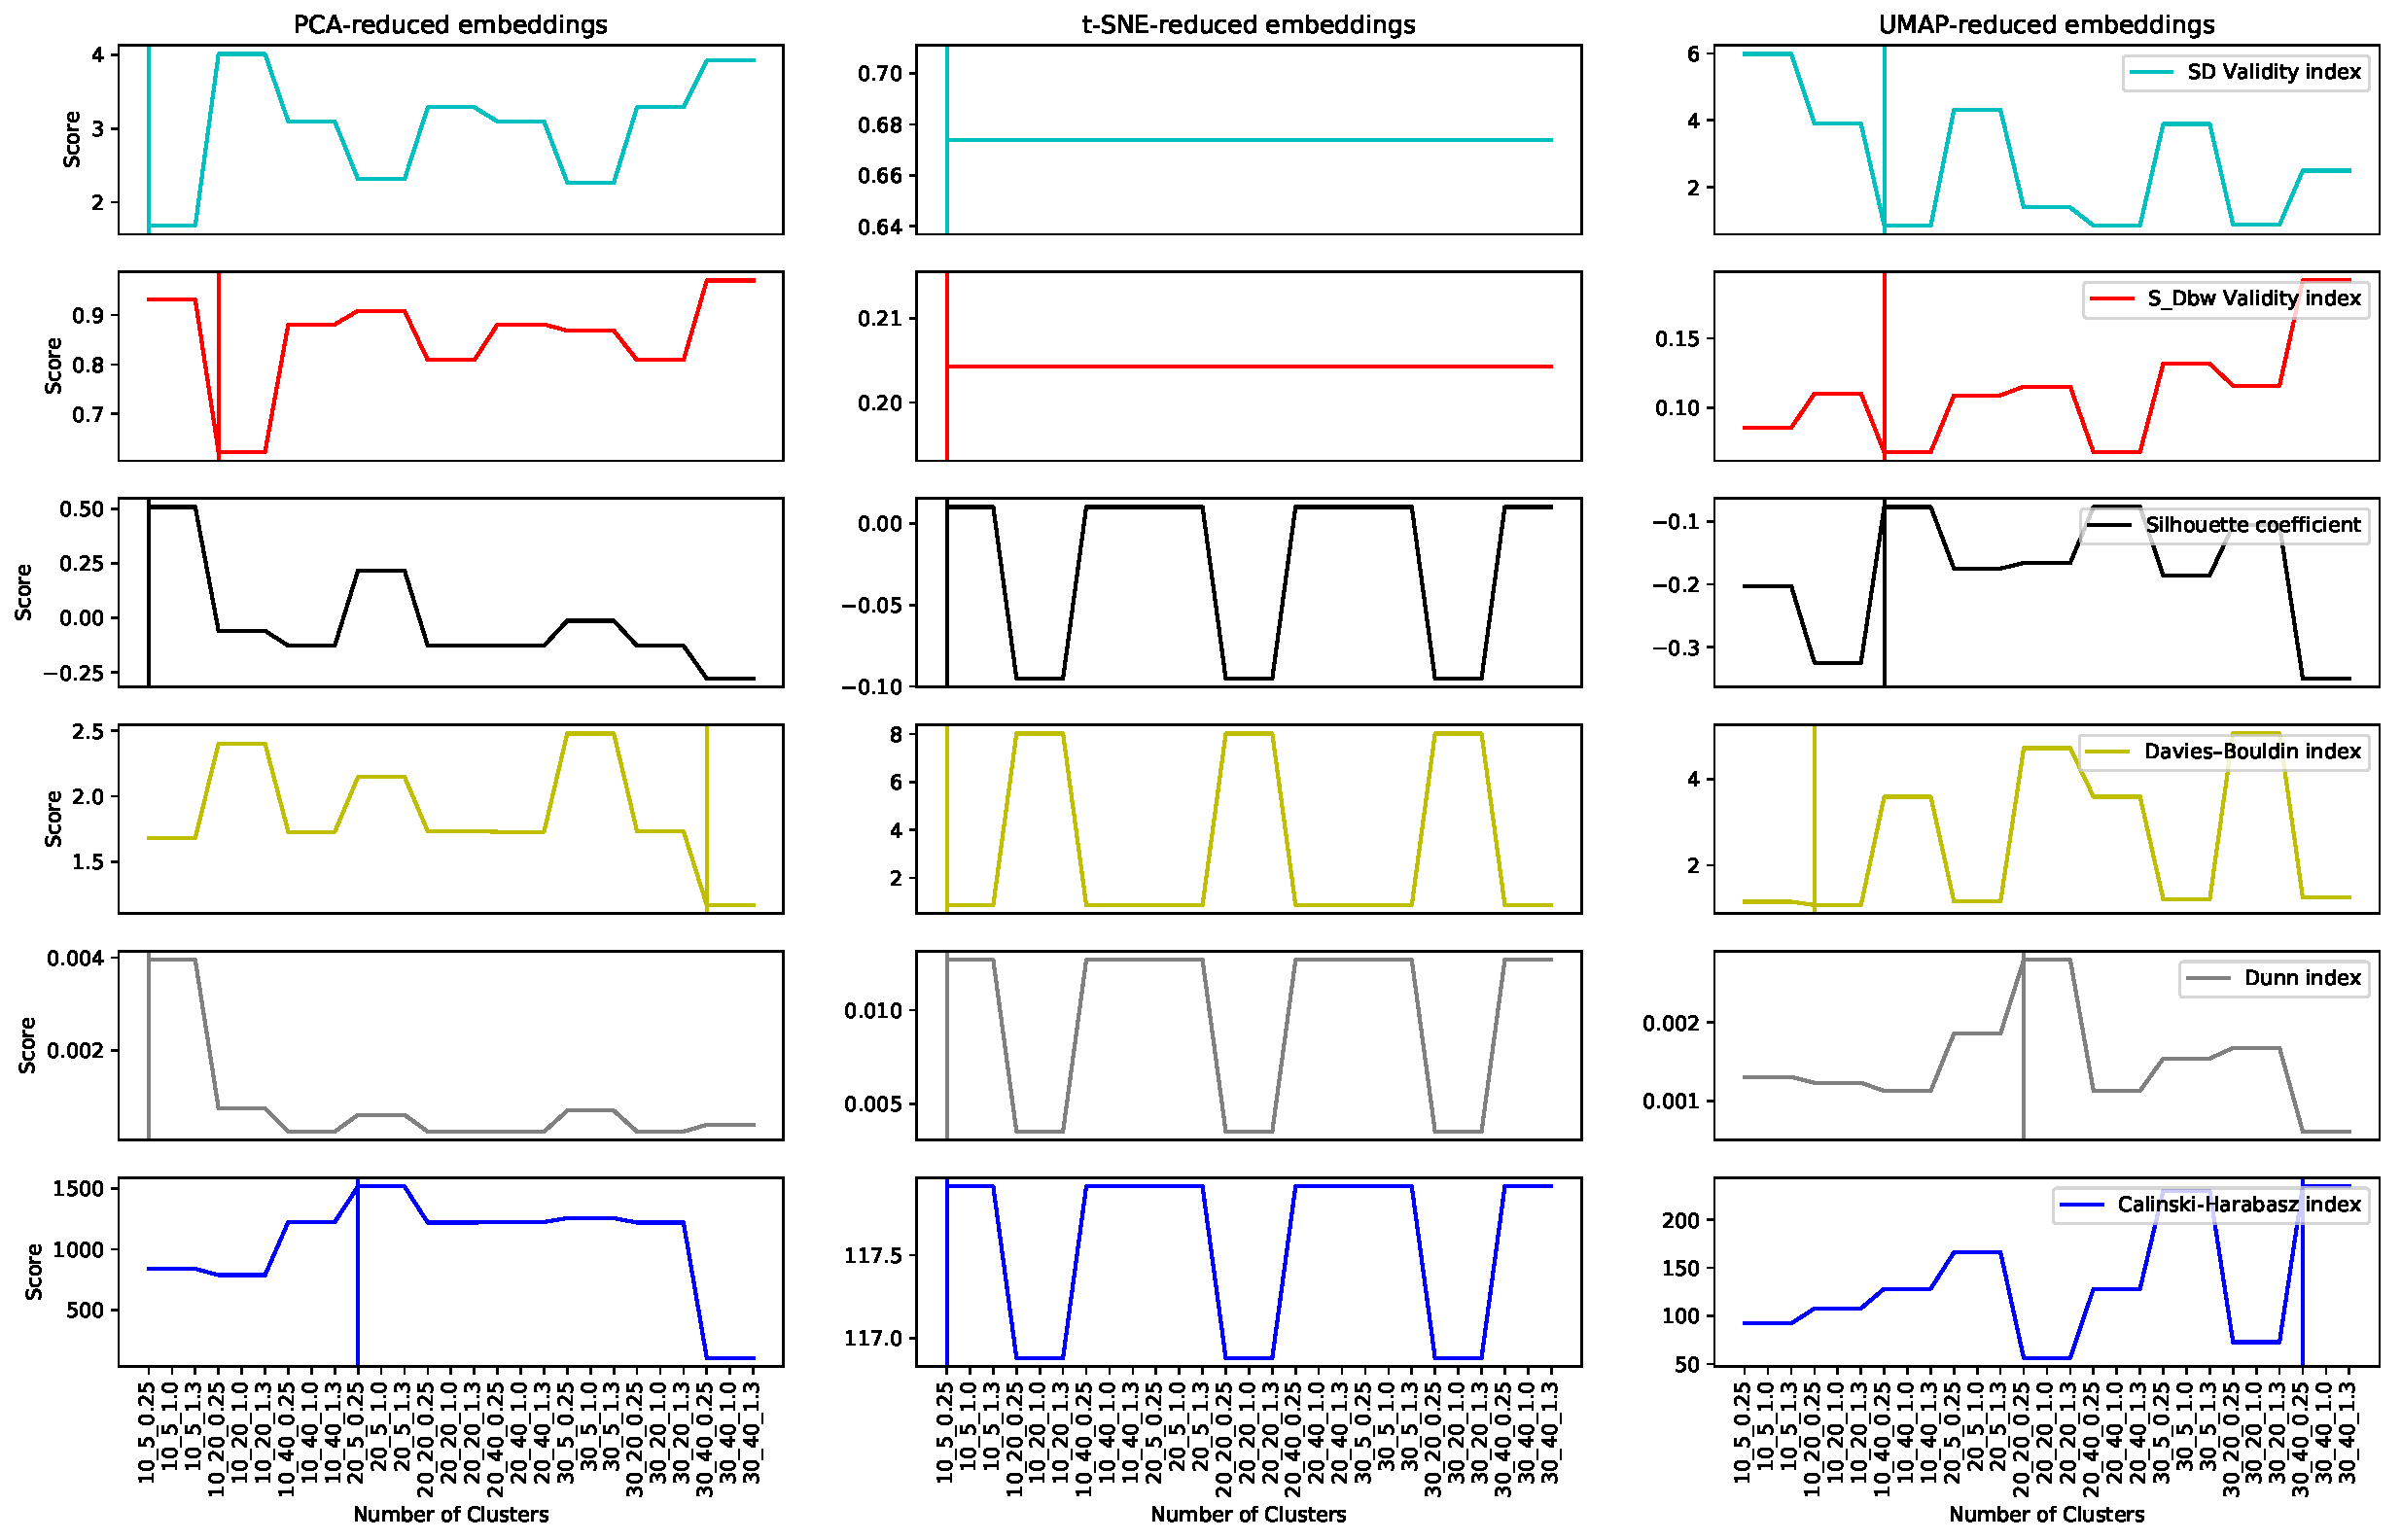
\includegraphics[width=1.0\textwidth]{images/appendix/App9.pdf}\\
	\caption{Evaluation of HDBSCAN clustering with respect to the set of hyperparameters.}
	\label{fig:App9}
\end{figure}
\begin{figure}[!ht]
	\centering
	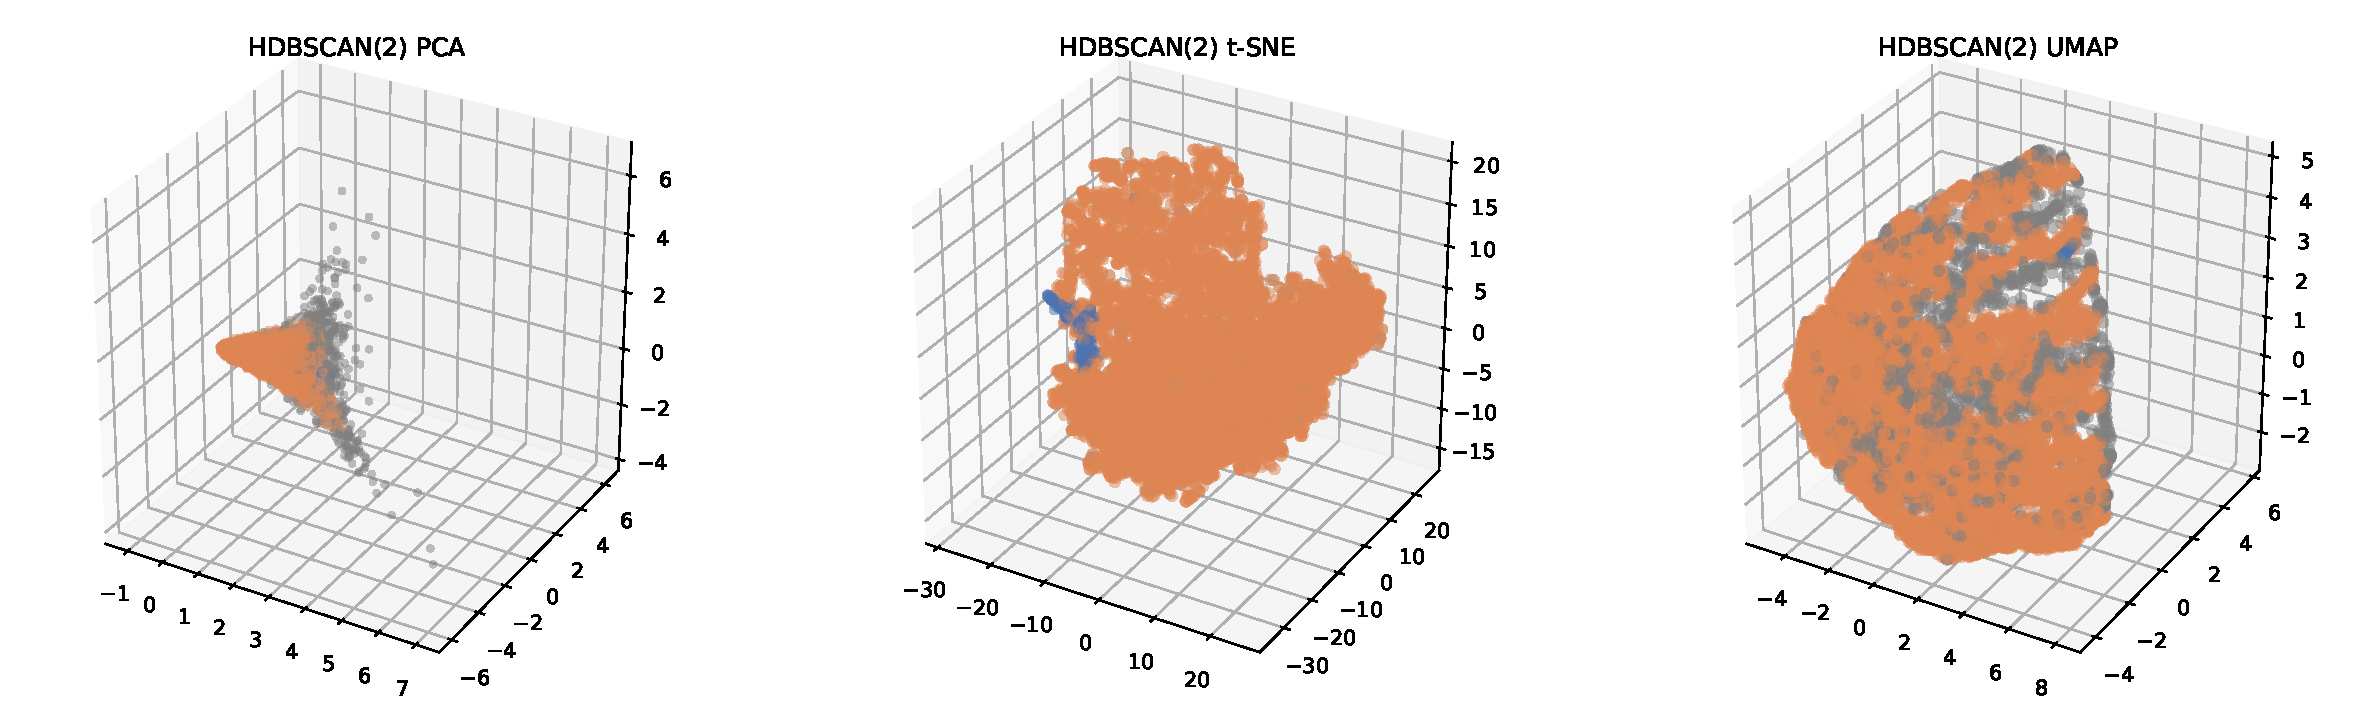
\includegraphics[width=1.0\textwidth]{images/appendix/App10.pdf}\\
	\caption{Resulting HDBSCAN clustering.}
	\label{fig:App10}
\end{figure}

\section{Interpretation of the results}
Some initial time analysis is needed to get an idea about overall time distribution in the network. The continuous period of explored part of the network spans approximately 13 months so that 26 consecutive time classes were allocated each of length of ~15 days. It is turned out that some of the users were active during several time classes, whereas the majority belong to only one class.~\autoref{fig:App13} shows the number of nodes by the number of time classes when they were active. Out of more than 11k nodes, almost 5k belong to more than one time classes.

\begin{figure}[!ht]
	\centering
	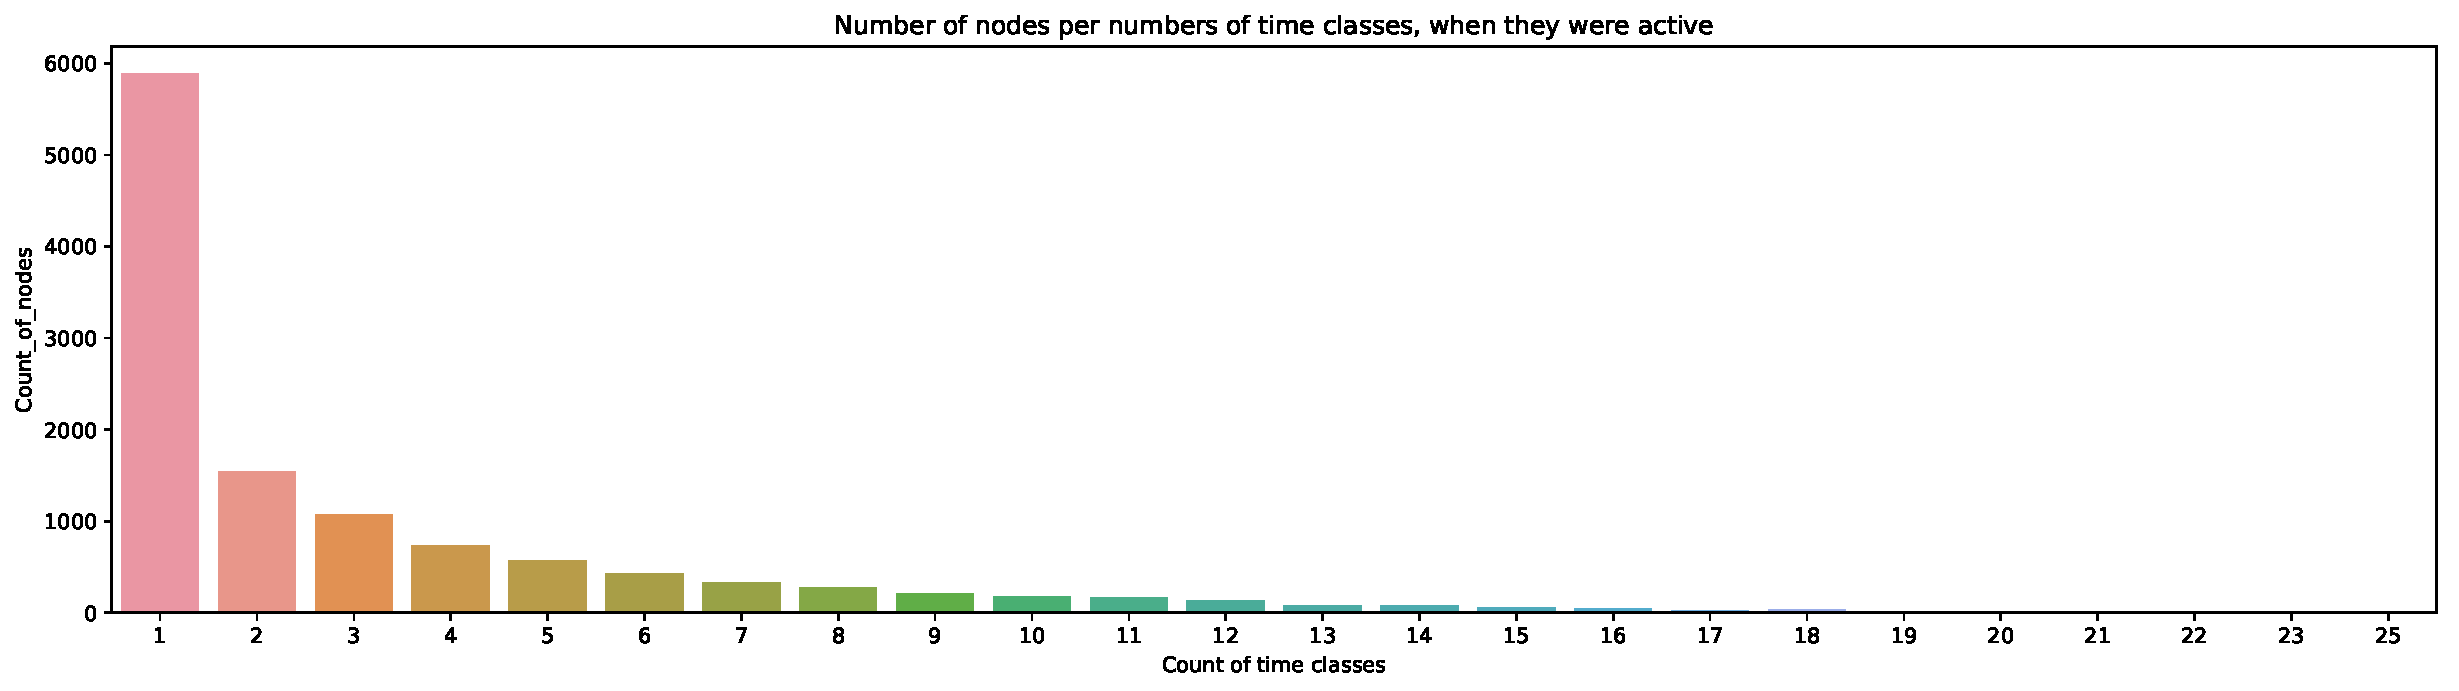
\includegraphics[width=1.0\textwidth]{images/appendix/App13.pdf}\\
	\caption{Number of nodes in the network by the number of time classes.}
	\label{fig:App13}
\end{figure}

A node, which was active in several time classes, is assigned to the class when it sent and received most transfers.~\autoref{fig:App14} describes how many nodes were the most active in every time class.

\begin{figure}[!ht]
	\centering
	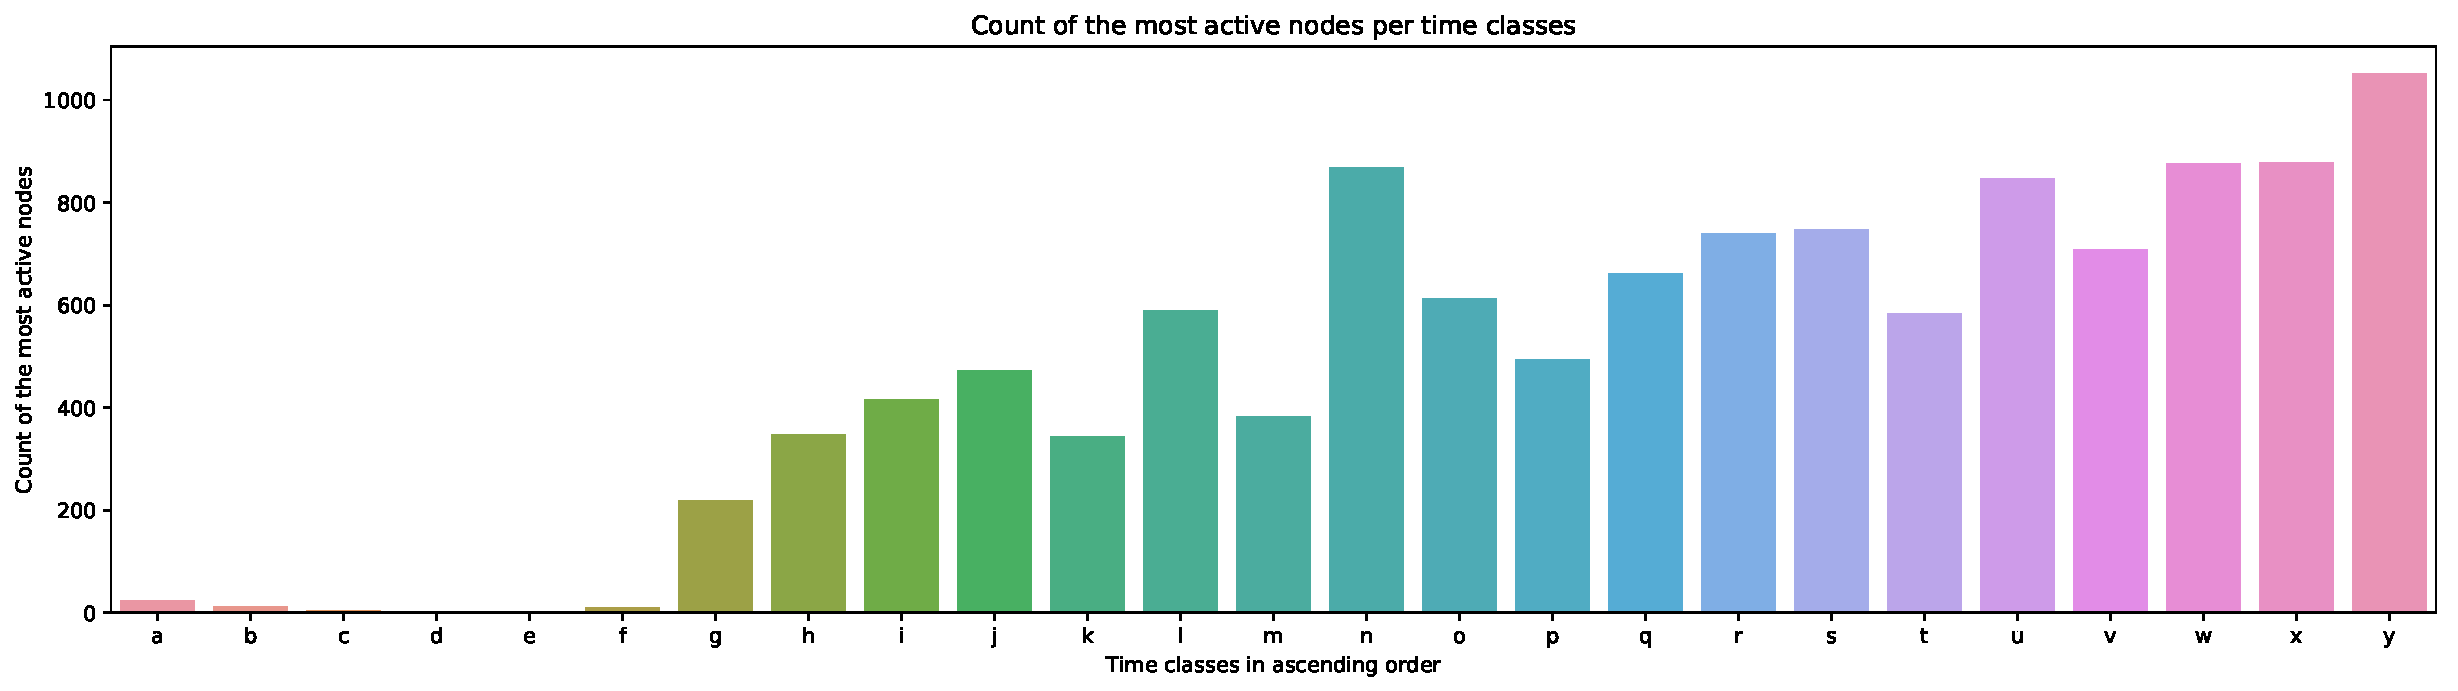
\includegraphics[width=1.0\textwidth]{images/appendix/App14.pdf}\\
	\caption{Count of the most active nodes per time class.}
	\label{fig:App14}
\end{figure}

~\autoref{fig:App15} provides a close look at the clusters produces by k-means. The numbers of nodes in each cluster are 3362, 3591, and  4926 from top to bottom respectively. From the figure it can be seen that the first cluster slightly overlaps with the second in terms of when users of each cluster were active. The first cluster consists of users mostly active by the end of the period. The users of the second cluster were the most active earlier in time and almost stop operating later on.  The third cluster unites nodes active over the entire period. The first six periods are naturally almost empty for all clusters because of the overall nodes distribution by time classes on~\autoref{fig:App14}.

\begin{figure}[!ht]
	\centering
	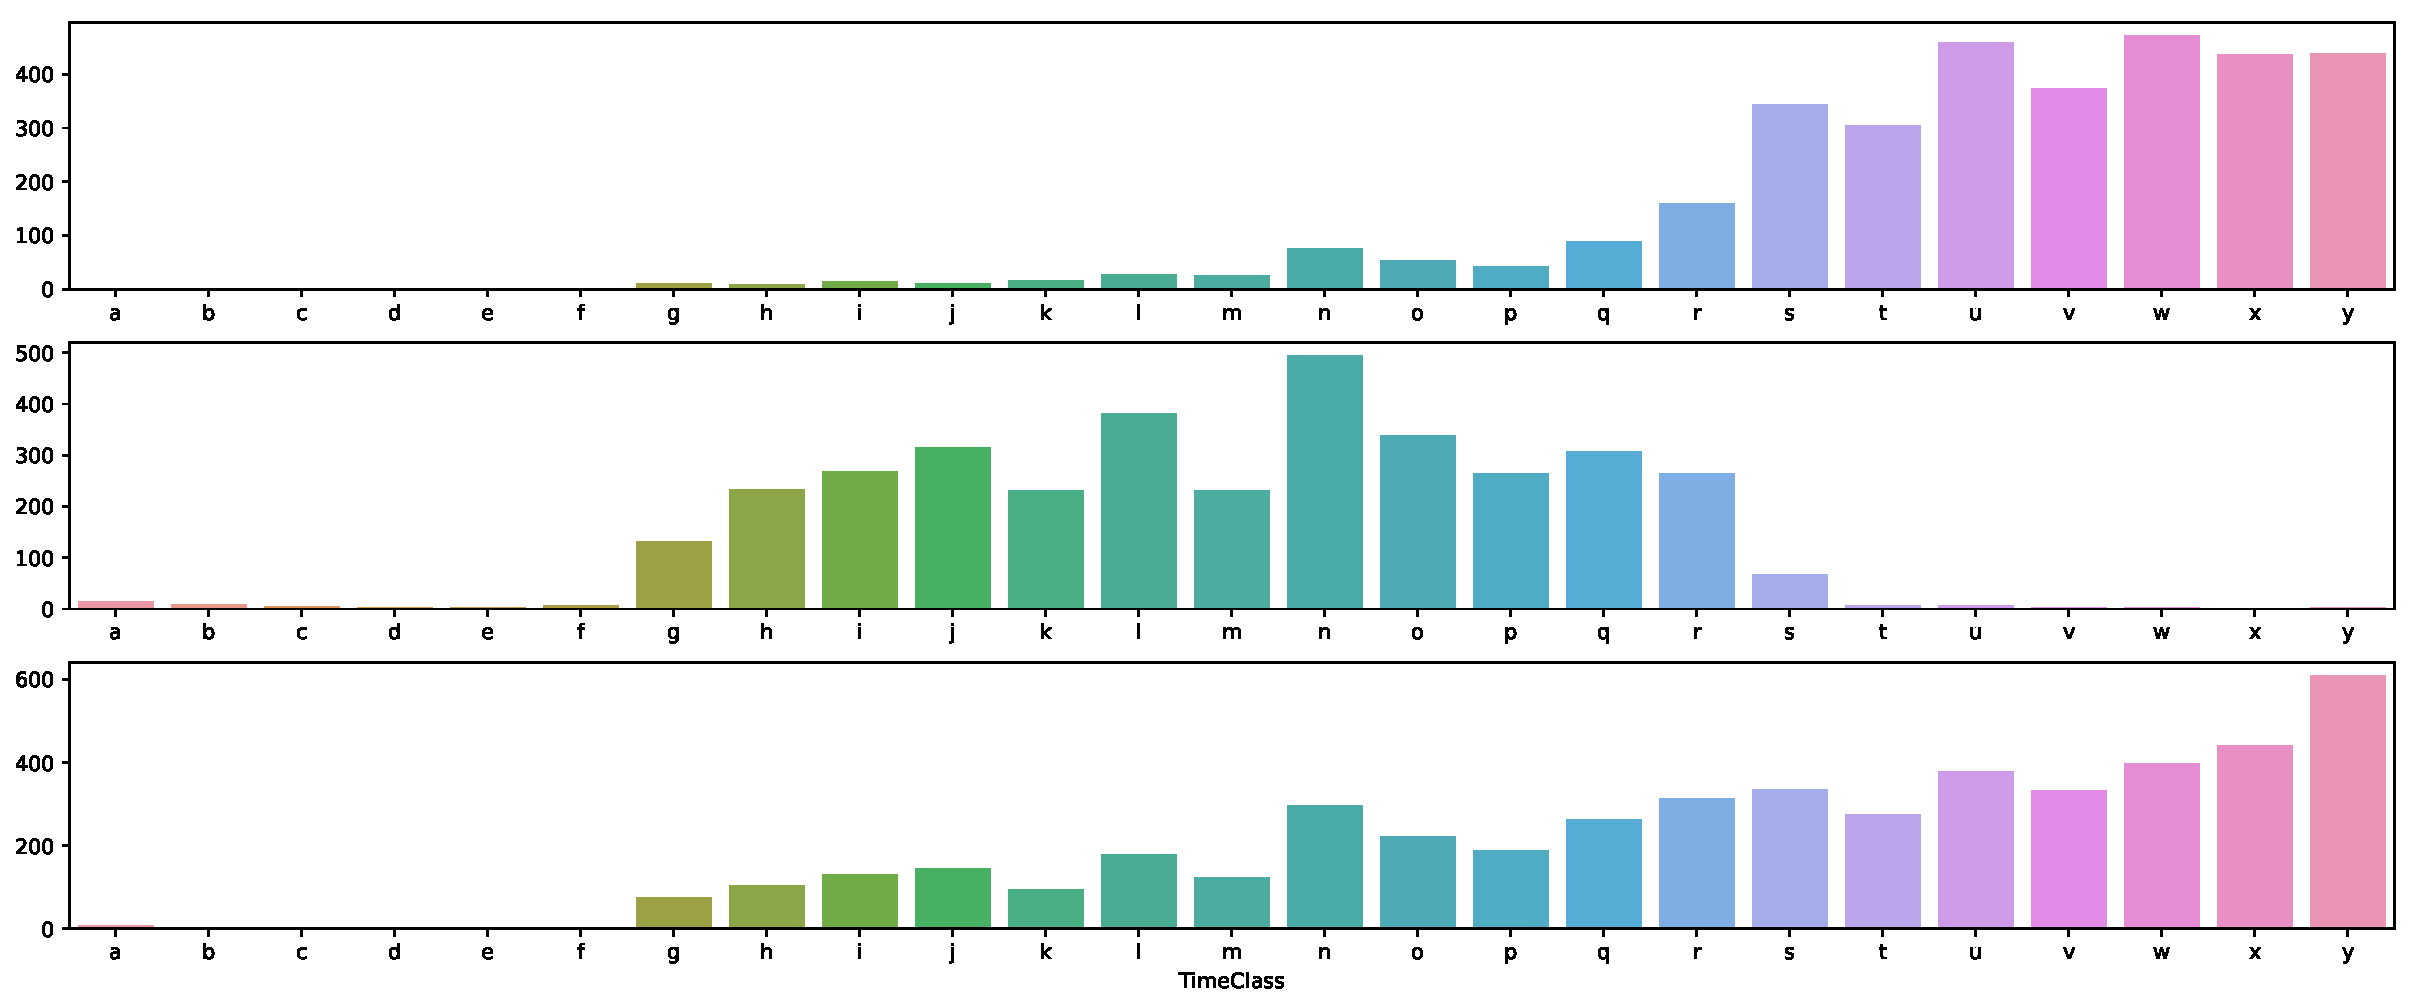
\includegraphics[width=1.0\textwidth]{images/appendix/App15.pdf}\\
	\caption{Time classes distribution of nodes in 3 $k$-means defined clusters in UMAP-redused set. From the first to the third cluster top to bottom.}
	\label{fig:App15}
\end{figure}

A very interesting embedding pattern produces t-SNE from the set of embeddings. The distribution of time classes within 2 HDBSCAN clusters (137 and 11741 nodes) is depicted on~\autoref{fig:App16}. It is notable that some group of users have been operating within each other over time classes l-m as they are connected also by local structural component.

\begin{figure}[!ht]
	\centering
	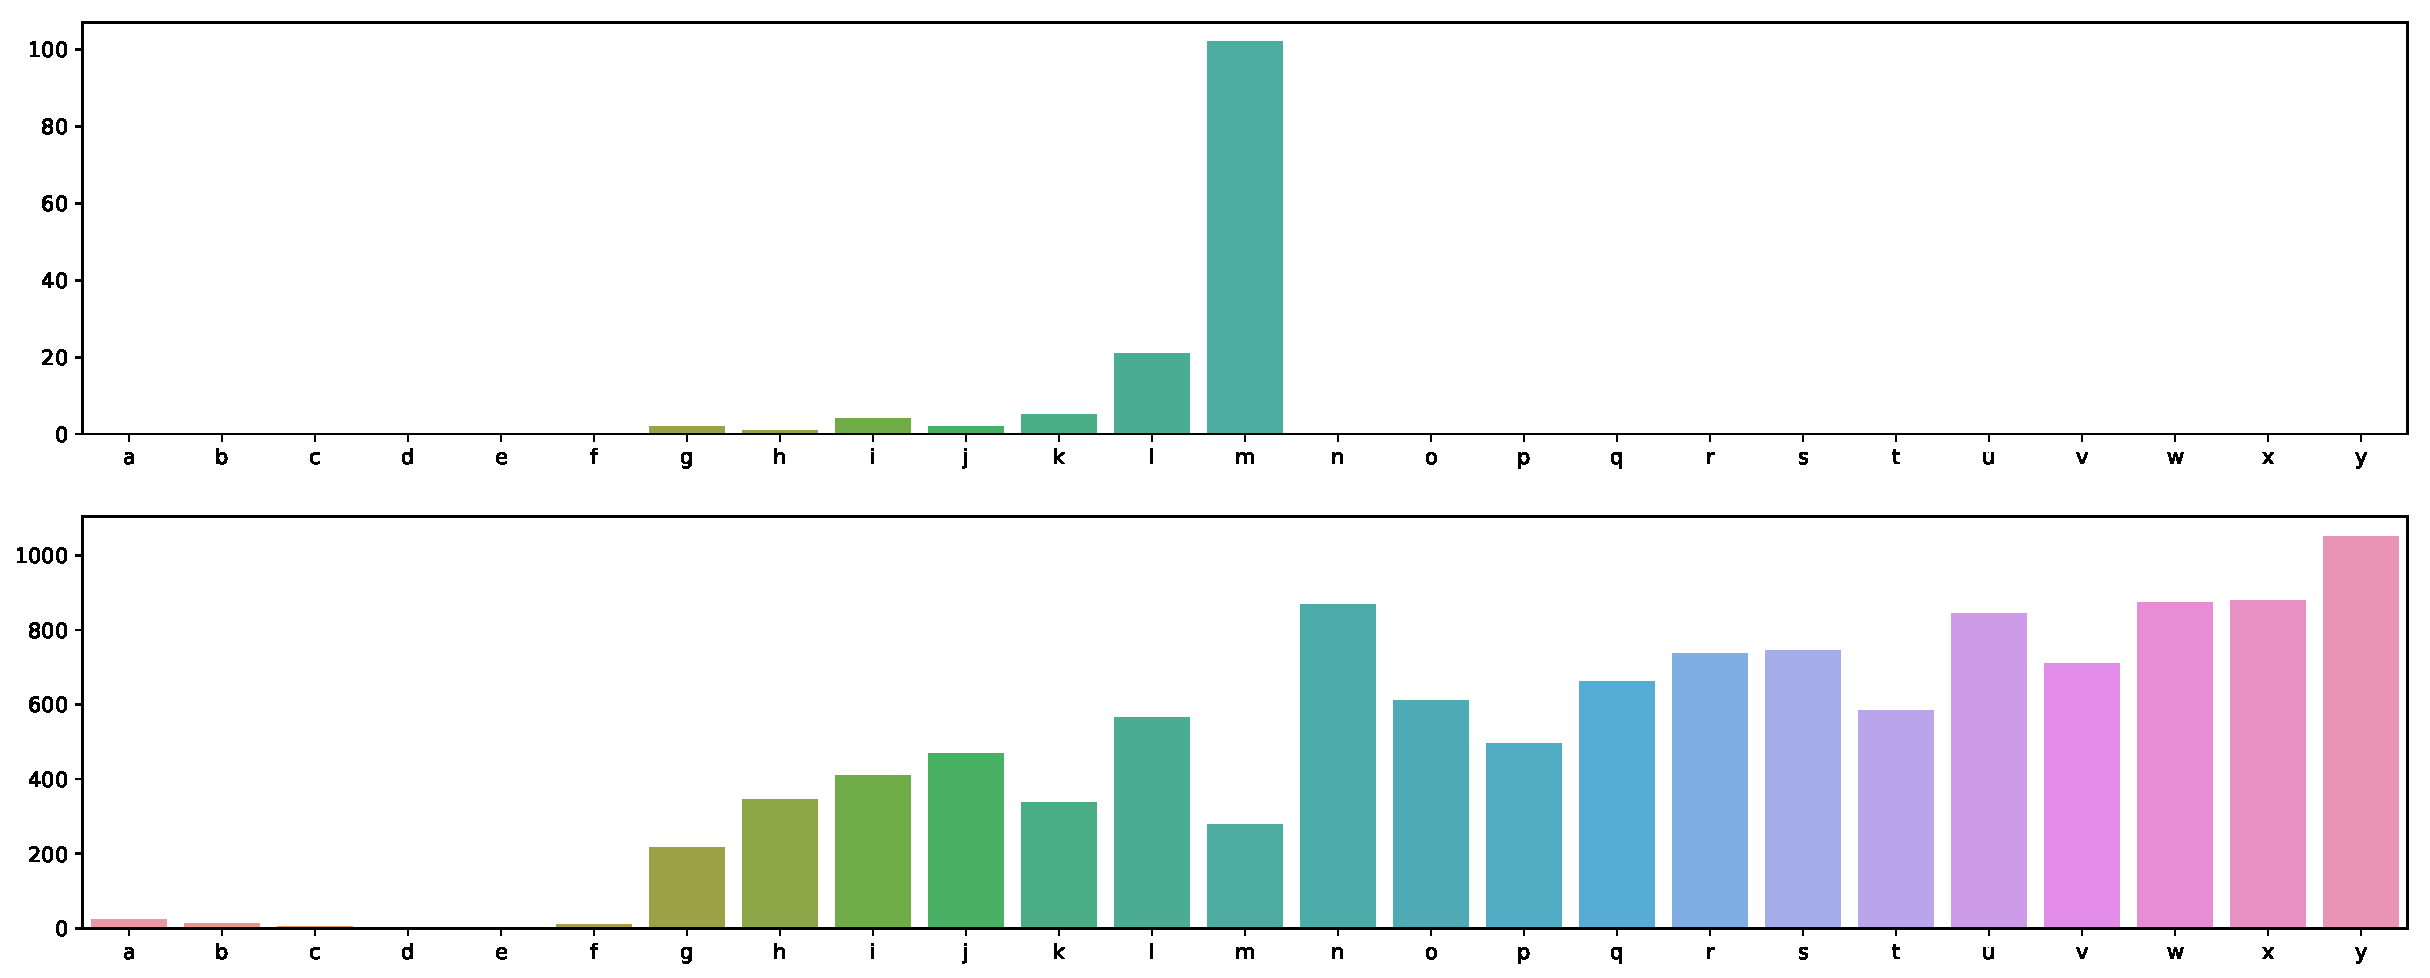
\includegraphics[width=1.0\textwidth]{images/appendix/App16.pdf}\\
	\caption{Time classes distribution of nodes in 2 HDBSCAN defined clusters in t-SNE-redused set. From the first to the second cluster top to bottom.}
	\label{fig:App16}
\end{figure}
